\chapter{Background\label{cha:background}}
In this chapter, we discuss the work our work builds on to give our work context. We cover the history of neural networks in machine learning, previous architectures that have been used to solve similar problems and the components of the solution we arrived at.  

\section{Neural Networks}
Artificial Neural Networks (ANNs), generally known as just Neural Networks (NNs) were first theorized in the 1940s \cite{mcculloch_logical_1943}. They are supposed to emulate the function of biological brains. They are composed of \enquote{neurons} which, when they receive a signal, apply a function to the signal which they then relay to the next neuron. Neural networks are built in layers. A layer receives a tensor of input values, each neuron in the layer takes a weighted sum of the inputs and applies its activation function to the result. These values are then passed on to the next layer. Training a neural network is the process of optimizing the weights in the layers of the network such that a specified input yields the desired output via iteration to minimize the output of a loss function \cite{goodfellow_deep_2016}.\\
Frank Rosenblatt created the perceptron in the 1950s. A perceptron is a single layer of neurons with the ability to classify images a few hundred pixels in size. Rosenblatt's breakthrough idea was to train a neural network based on reinforcement from a dataset, strengthening successful connections and weakening unsuccessful connections. His training algorithm was very limited and so inefficient that it did not allow for neural networks with more than one layer \cite{rosenblatt_perceptron_1958}. Based on his work, Rosenblatt first theorized the ability of neural networks to recognize people and translate between languages \cite{vandeput_brief_nodate}.\\
In 1974 Paul Werbos proposed backpropagation to optimize neural networks \cite{Werbos:74}, which became popular in 1986  with the work of Rumelhart et al. \cite{rumelhart_learning_1986}.  Backpropagation is an efficient training algorithm opening up the possibility of training neural networks deeper than one layer using gradient descent. \enquote{The backpropagation algorithm works by computing the gradient of the loss function with respect to each weight by the chain rule, computing the gradient one layer at a time, iterating backward from the last layer to avoid redundant calculations of intermediate terms in the chain rule} \cite{noauthor_backpropagation_2022}. Backpropagation enabled the creation of deeper neural networks, notably used to read handwritten digits with good accuracy \cite{lecun_backpropagation_1989}.\\
Although backpropagation enabled neural networks with multiple layers, it did not enable significant depth. The most commonly used activation functions of the time, sigmoid and tanh, have derivatives close to zero, so stacking them flattens the gradient in the network values at an exponential rate. This slows down the gradient descent used to optimize the networks, also at an exponential rate. In the 2010s the ReLu activation function \cite{nair_rectified_2010} coupled with improved optimization algorithms like ADAM and massive advances in computer hardware opened the door for Deep Learning, neural networks with many more layers. Today, deep neural networks have been used to great effect in applications like Google DeepMind's AlphaGO \cite{silver_mastering_2016}, the first AI to beat the world champion in the game of go, and OpenAI's GPT3 model generates text human-like enough to pass the Turing test, to be confused with text written by a human \cite{vandeput_brief_nodate}.


\section{Recurrent Neural Networks\label{cha:RNN}}
Recurrent Neural Networks (RNNs), especially Gated Recurrent Units (GRUs) and Long Short-Term Memory (LSTM) cells \cite{Goodfellow-et-al-2016, hochreiter_long_1997} along with more advanced derivatives have been shown to be able to achieve good results when trained on previous weather and power generation data \cite{lin_temporal_2020, lee_forecasting_2018, jaidee_very_2019, su_machine_2019}.
RNNs are a class of deep neural networks where nodes are connected in a temporal sequence, allowing the network to learn time-based data efficiently \cite{lim_time_2021}. LSTMs and GRUs are types of RNNs in which, the nodes in the network have additional stored states controlled by the network via mechanisms that use time delays or feedback loops \cite{Goodfellow-et-al-2016, noauthor_recurrent_2021}. Figure~\ref{fig:RNNs} shows the structure of the nodes of the three different Recurrent Neural Network types discussed above.\\

\begin{figure}[ht!]
    \centering
    \subfloat[Plain Recurrent Neural Network (RNN)]{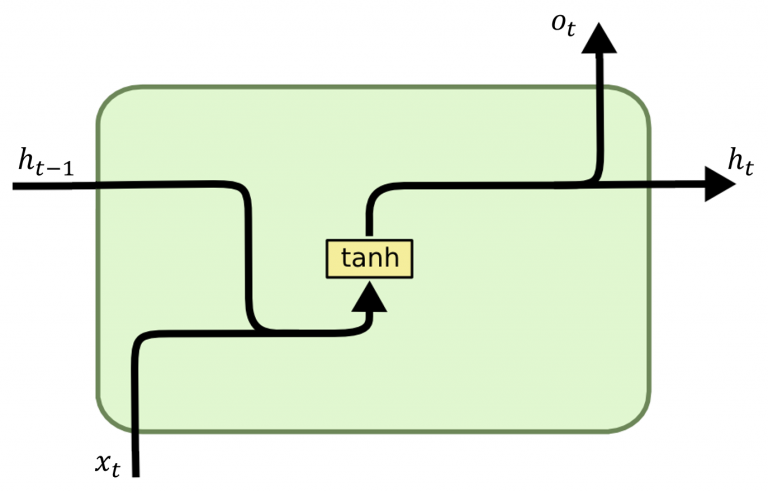
\includegraphics[scale=0.35]{imgs/RNN.png}\label{fig:RNN}}\qquad
    \subfloat[Gated Recurrent Unit (GRU)]{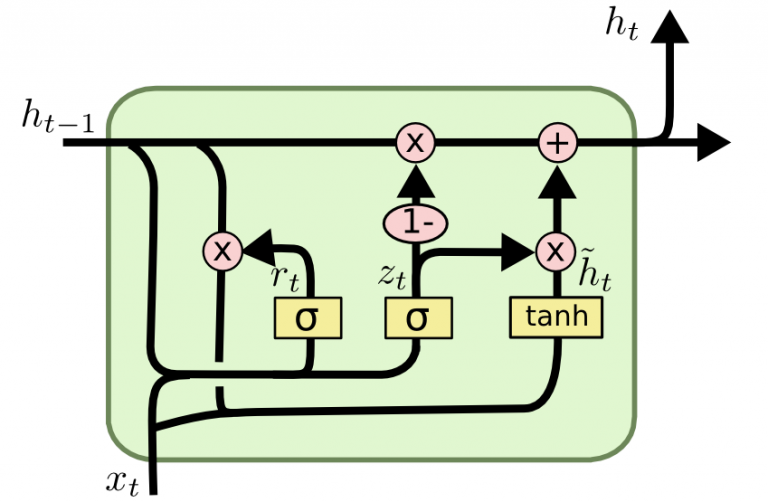
\includegraphics[scale=0.35]{imgs/GRU.png}\label{fig:GRU}}\qquad
    \subfloat[Long Short-Term Memory (LSTM)]{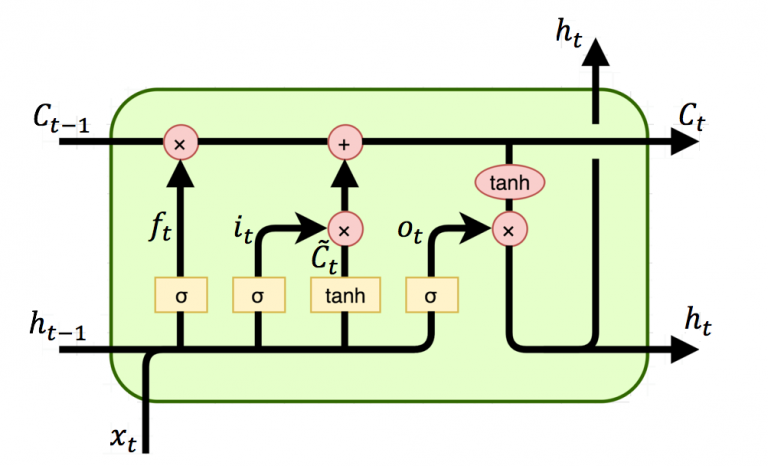
\includegraphics[scale=0.35]{imgs/LSTM.png}\label{fig:LSTM}}\qquad
    \caption{The cells of different Recurrent Neural Network types. $x_t$ represents inputs, $h_t$ and $C_t$ represent hidden layer vectors passed between cells. $\sigma$ and $tanh$ are activation functions. \cite{lopez_rnn_nodate}.
    \label{fig:RNNs}}
\end{figure}

%\ifdraft{Provide background about the subject matter (e.g. How was morse code
%developed?  How is it used today?). 
%This is a place where there are usually many citations.
%It is suspicious when there is not.
%Include the purpose of the different equipment and your design intent. 
%Include references to relevant scientific/technical work and books.
%What other examples of similar designs exist?
%How is your approach distinctive?

%If you have specifications or related standards, these must be
%described and cited also.  As an example, you might cite the specific
%RoboSub competition website (and documents) if working on the lighting system for an AUV\cite{guls2016auvlight}


\section{Transformers\label{cha:transformer}}
%Hard to train
%sequential
% -> parallelization hard
%encoder/decoder instead. Attention. 
% Explain enc/dec
% Autoencoders generate same output as the input, so no labeled data is needed -> completely unsupervisd earning.
% Locality a problem with CNNs and RNNs. Can easily find local context but keeping on to context far apart in input is difficult. Enter transformers.
 %Encoder reads blocks of data and uses that and previously generated data as inputs into decoder which generatesdata one point at a time.
 %Attention. How you relate things to each other. i.e. input to output
 %self attention. How do features in the input data relate to each other
 
Transformers have been used for a while in Natural Language Processing (NLP) and have more recently been used very effectively in forecasting \cite{vaswani_attention_2017}. They can more effectively learn and preserve local context located far apart in the input data. As an example from NLP, the training data can contain multiple cases where time is being told, far apart. A transformer model would then more easily identify that the word \enquote{o’clock} is generally preceded by a number, whereas RNNs would be more likely to struggle with such distributed information. This can be applied to our work as similar weather patterns would reoccur days apart and cause a similar effect on measured irradiance at the power station \cite{lim_time_2021}. Figure~\ref{fig:transformer} shows an overview of the transformer architecture.

\afterpage{%
\begin{figure}
    \centering
    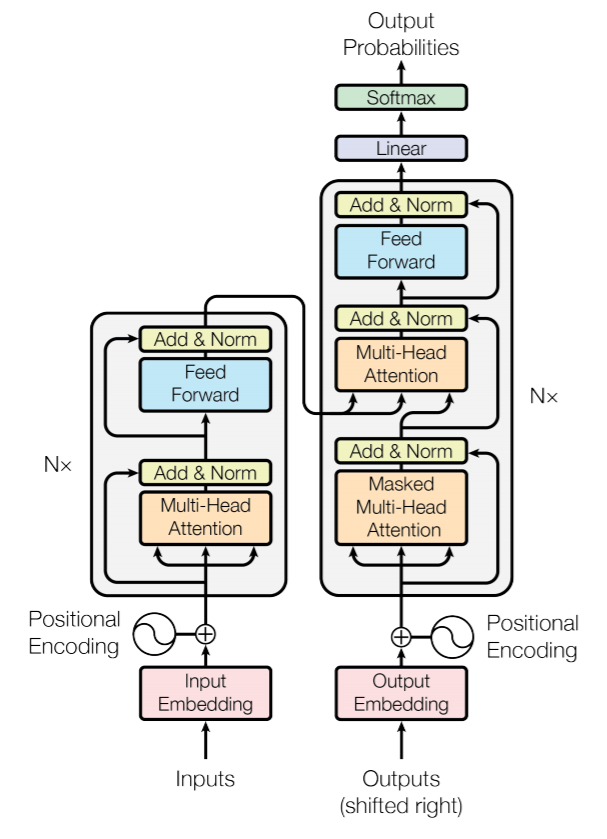
\includegraphics[scale=0.80]{imgs/transformer.png}
    \caption{The transformer architecture.\cite{vaswani_attention_2017}
    \label{fig:transformer}}
\end{figure}
\clearpage
}



\subsection{Encoder/decoder}
Transformers have an encoder/decoder structure, depicted in Figure~\ref{fig:encoder_decoder}. An encoder takes an input sequence and generates an abstract hidden state which the decoder then uses to generate an output sequence \cite{vaswani_attention_2017}. A major advantage of this methodology is that the inputs and outputs do not have to have the same length, whereas the primary limit of the architecture is that all information in the input sequence needs to be represented by a single vector for the decoder to decode. The encoder distils the input down to a much smaller representation, a bottleneck, only containing desired information which the decoder in turn extracts. This is on its own used for tasks like de-noising or colourizing images \cite{nechu_what_2020}. 

\begin{figure}
    \centering
    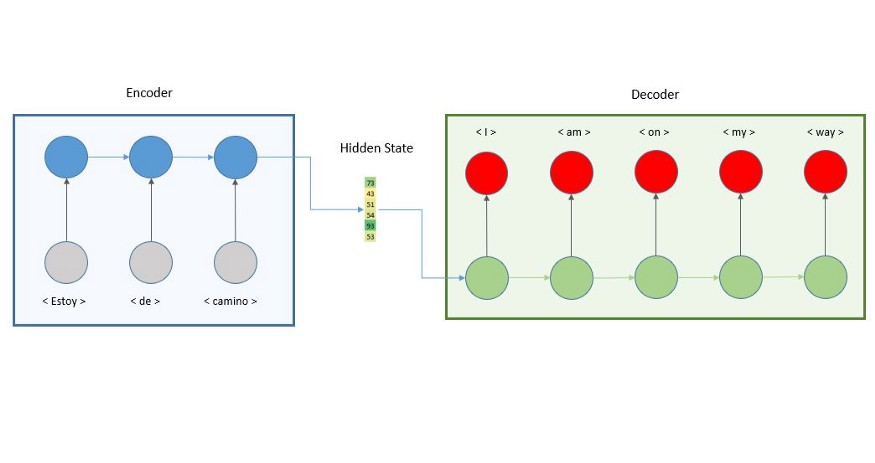
\includegraphics[scale=0.5]{imgs/encoder_decoder.jpeg}
    \caption{The encoder/decoder structure \cite{nechu_what_2020}
    \label{fig:encoder_decoder}}
\end{figure}

\subsection{Positional encoding}
Unlike RNNs, the transformer architecture has no recurrence, or cell based memory, and does not inherently track the order of the input data, so positional information has to be injected into the network input for the model to be able to use the positional context of the data.\cite{vaswani_attention_2017}

\subsection{Self-attention} We previously discussed transformers' ability to preserve context across the long input sequences. That is thanks to the attention layer. The attention layer encodes an input data point's relevance to the rest of the points in the input sequence. Calling back to the previous NLP example, it encodes the context that the word \enquote{o'clock} is relevant to numbers because it is preceded by a number in most inputs.
 
A single attention head can put all the focus on a single element. Multiple attention heads can be used to let the transformer model consider the context of more elements at the same time \cite{rohrer_transformers_2021}.

\section{Weather forecasts\label{cha:WRF}}
Numerical Weather Prediction (NWP) has used mathematical models of the oceans and atmosphere since the 1920s to predict the weather based on current conditions, although realistic results weren't achieved until the advent of computer simulations in the 1950s \cite{noauthor_numerical_2022}. The Weather Research and Forecasting (WRF) model is an NWP system created by the National Center for Atmospheric Research (NCAR), the National Oceanic and Atmospheric Administration (NOAA), the Air Force Weather Agency (AFWA), the Naval Research Laboratory (NRL), the University of Oklahoma (OU), and the Federal Aviation Administration (FAA) in the United States for both research and operational weather forecasting \cite{noauthor_weather_2022}.\\
WRF-SOLAR is an NWP model based on WRF specifically designed to model values useful for solar power, including high frequency irradiance calculations, more accurate solar position algorithms, and more robust aerosol and particle simulations with regard to radiation \cite{jimenez_wrf-solar_2016}.
\section{Previous work}
Lin et al. \cite{lin_temporal_2020} showed that while the more traditional GRUs and LSTMs show good performance on the task, Temporal Convolutional Neural Networks (TCNN) can show even better performance. \textit{\endquote{TCNN is a novel convolutional architecture designed for sequential modelling, which combines causal and dilated convolutions
and residual connections}} \cite{lin_temporal_2020}. \\
Jaidee et al. \cite{jaidee_very_2019} showed that LSTMs, GRUs and derivative methods show relatively similar performance for very short-term predictions on the time scale of a few hours. This timescale is where it is critical to accurately predict cloud movements. 
These methods have been taken as far as building genetic algorithms to generate the optimal neural network for the purpose \cite{jaidee_very_2019}. These genetic algorithms operate on the same principles as animal breeding. They generate multiple candidate neural networks and use the best networks as a base to generate new networks for the next generation. This is done for multiple generations and in the end, the best neural network generated is used \cite{jaidee_very_2019}.\\
Su et al. \cite{su_machine_2019} did extensive experimentation on more conventional neural networks and newer, less known networks including  Non-linear Auto Regressive Neural Networks (NARXNN), as well as various statistical approaches. When predicting power output, NARXNN takes in the current power output values and considers them, in real time, as well as the past values of the power output of the system. These experiments showed that NARXNN had the best performance of these, by a rather large margin, and a hybrid method, of the better performing methods, showed even better results \cite{anderson_using_2018}. The statistical methods generally performed significantly worse in predicting the power output. \\
Satellite imagery has been used for predicting solar power output as well. A neural network was trained to predict solar power production, primarily from cloud cover information it learned from these satellite images \cite{jang_solar_2016}.\\
\textcolor{red}{AlexNet}